\begin{minipage}[c]{\textwidth}
\advance\leftskip-2.5cm
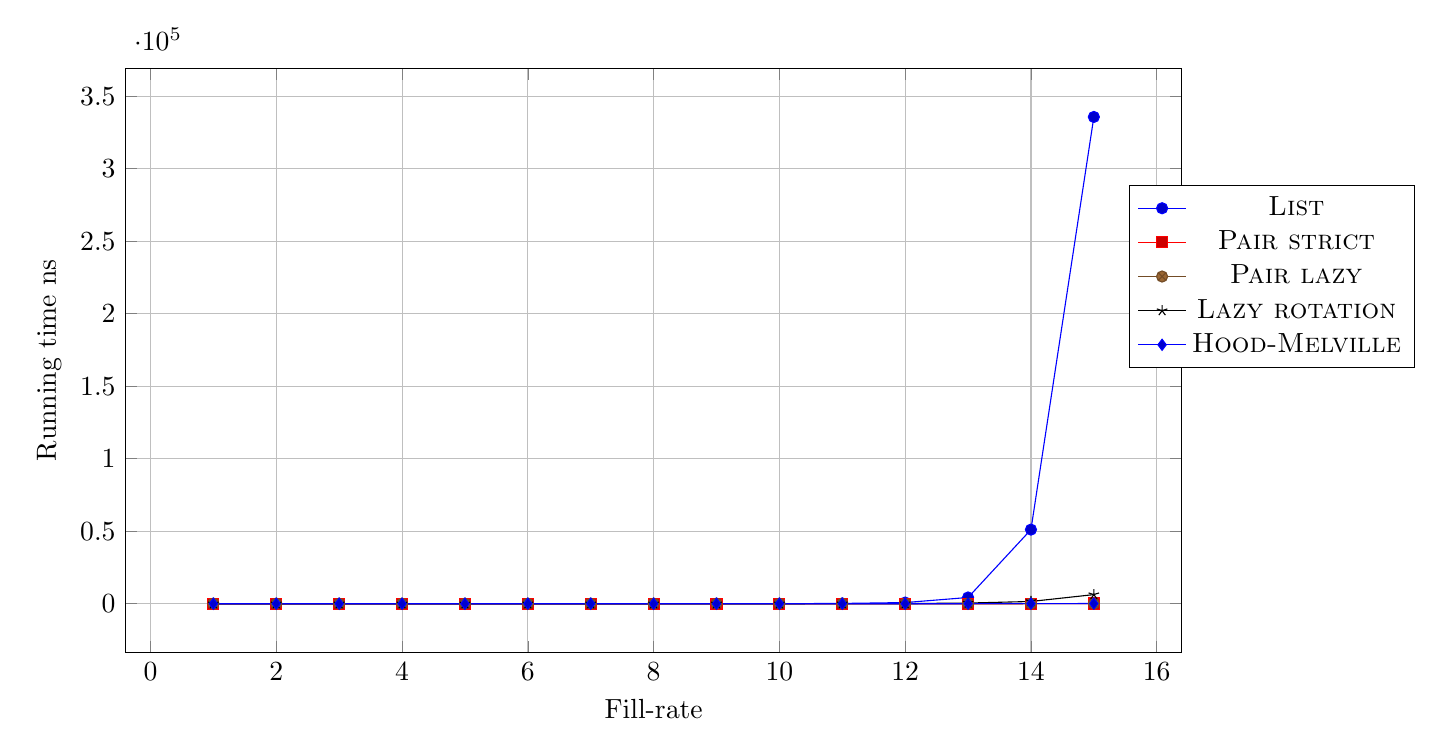
\begin{tikzpicture}
        \begin{axis}[
            xlabel = Fill-rate,
            ylabel = Running time ns,
            height=9cm,
            width=15cm,
            grid=major,
            legend style={
            at={(0.95,0.8)},
            anchor=north west}]            
            legend pos=center west
    	]
    		
    		
    	\addplot coordinates {
(1,0)
(2,0)
(3,0)
(4,0)
(5,0)
(6,0)
(7,2)
(8,20)
(9,56)
(10,23)
(11,199)
(12,805)
(13,4308)
(14,51122)
(15,335703)

    	};
        
    	\addlegendentry{\textsc{List}}

                \addplot coordinates {
(1,0)
(2,0)
(3,0)
(4,0)
(5,0)
(6,0)
(7,0)
(8,1)
(9,0)
(10,2)
(11,4)
(12,9)
(13,3)
(14,23)
(15,127)

    	};
        
    	\addlegendentry{\textsc{Pair strict}}

        \addplot coordinates {
(1,0)
(2,0)
(3,0)
(4,0)
(5,0)
(6,0)
(7,0)
(8,1)
(9,0)
(10,2)
(11,4)
(12,9)
(13,3)
(14,23)
(15,127)

    	};
        
    	\addlegendentry{\textsc{Pair lazy}}

        \addplot coordinates {
(1,0)
(2,0)
(3,0)
(4,0)
(5,0)
(6,0)
(7,0)
(8,0)
(9,-3)
(10,8)
(11,39)
(12,124)
(13,459)
(14,1556)
(15,6288)

    	};
        
    	\addlegendentry{\textsc{Lazy rotation}}

        \addplot coordinates {
(1,0)
(2,0)
(3,0)
(4,0)
(5,0)
(6,0)
(7,0)
(8,1)
(9,0)
(10,7)
(11,12)
(12,11)
(13,19)
(14,59)
(15,140)

    	};
        
    	\addlegendentry{\textsc{Hood-Melville}}

        \end{axis}

    \end{tikzpicture}
    \captionof{figure}{TITEL}
    \label{fig:sample_figure}
\end{minipage}